% Created 2024-04-21 dom 08:40
% Intended LaTeX compiler: pdflatex
\documentclass[aspectratio=169, usenames,svgnames,dvipsnames]{beamer}
\usepackage[utf8]{inputenc}
\usepackage[T1]{fontenc}
\usepackage{graphicx}
\usepackage{longtable}
\usepackage{wrapfig}
\usepackage{rotating}
\usepackage[normalem]{ulem}
\usepackage{amsmath}
\usepackage{amssymb}
\usepackage{capt-of}
\usepackage{hyperref}
\usepackage{color}
\usepackage{listings}
\usepackage{mathpazo}
\usepackage[spanish]{babel}
\usepackage{gensymb}
\usepackage{amsmath}
\usepackage{diffcoeff}
\usepackage{steinmetz}
\usepackage{mathtools}
\bibliographystyle{plain}
\usepackage{siunitx}
\sisetup{output-decimal-marker={,}}
\DeclareSIUnit{\watthour}{Wh}
\hypersetup{colorlinks=true, linkcolor=Blue, urlcolor=Blue}
\usepackage[symbol, perpage]{footmisc}
\newcommand{\laplace}[1]{\mathbf{#1}(\mathbf{s})}
\newcommand{\slp}{\mathbf{s}}
\newcommand{\fasor}[1]{\mathbf{#1}(\omega)}
\newcommand{\atan}{\mathrm{atan}}
\parskip=5pt
\usetheme{Boadilla}
\usecolortheme{rose}
\usefonttheme{serif}
\author{Oscar Perpiñán Lamigueiro}
\date{}
\title{Acoplamientos Magnéticos}
\subtitle{Teoría de Circuitos II}
\setbeamercolor{alerted text}{fg=blue!50!black} \setbeamerfont{alerted text}{series=\bfseries}
\AtBeginSubsection[]{\begin{frame}[plain]\tableofcontents[currentsubsection,sectionstyle=show/shaded,subsectionstyle=show/shaded/hide]\end{frame}}
\AtBeginSection[]{\begin{frame}[plain]\tableofcontents[currentsection,hideallsubsections]\end{frame}}
\beamertemplatenavigationsymbolsempty
\setbeamertemplate{footline}[frame number]
\setbeamertemplate{itemize items}[triangle]
\setbeamertemplate{enumerate items}[circle]
\setbeamertemplate{section in toc}[circle]
\setbeamertemplate{subsection in toc}[circle]
\hypersetup{
 pdfauthor={Oscar Perpiñán Lamigueiro},
 pdftitle={Acoplamientos Magnéticos},
 pdfkeywords={},
 pdfsubject={},
 pdfcreator={Emacs 29.2 (Org mode 9.6.23)}, 
 pdflang={Spanish}}
\begin{document}

\maketitle

\section{Bobina}
\label{sec:orgdea8fa4}

\begin{frame}[label={sec:org02f4857}]{Ley de Ampere}
Una corriente eléctrica circulando por un conductor crea un campo magnético en torno al conductor (\emph{regla de la mano derecha})

\begin{center}
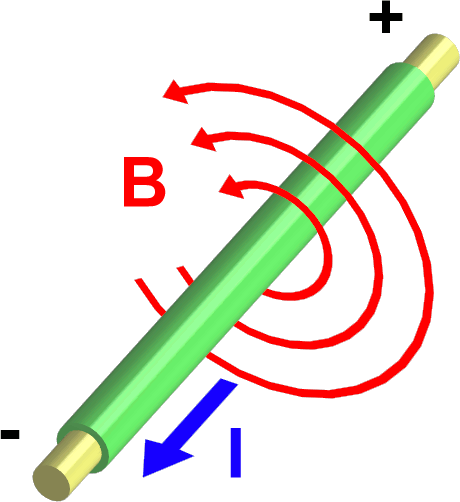
\includegraphics[height=0.7\textheight]{../figs/Electromagnetism.png}
\end{center}
\end{frame}


\begin{frame}[label={sec:org6316402}]{Ley de Faraday}
Cuando un \alert{campo magnético variable} atraviesa una espira \alert{estática} aparece una \alert{tensión inducida} \alert{proporcional al flujo} y opuesta a su variación.

\[
u(t) = \frac{\mathrm{d}\phi}{\mathrm{d}t} 
\]

El flujo magnético es la cantidad de líneas de fuerza magnética que atraviesan una superficie. 

\begin{columns}
\begin{column}{0.3\columnwidth}
\[
\phi = \vec{B} \cdot \vec{A} \ [\mathrm{Wb}]
\]
\end{column}

\begin{column}{0.7\columnwidth}
\begin{center}
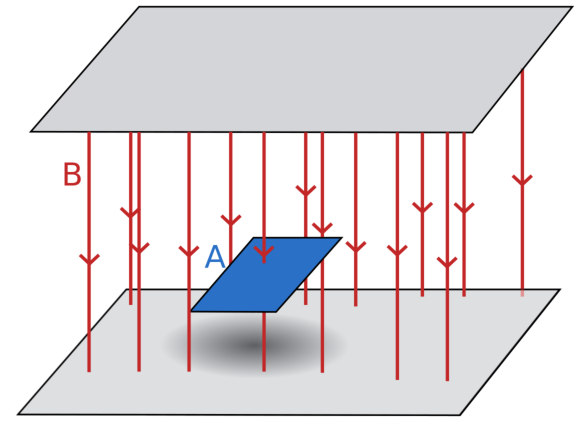
\includegraphics[height=0.45\textheight]{../figs/flujo_magnetico.pdf}
\end{center}
\end{column}
\end{columns}
\end{frame}

\begin{frame}[label={sec:orga3f6dbb}]{Bobina}
Una bobina es un arrollamiento de un conductor (\emph{conjunto de \(N\) espiras conectadas en serie}) alrededor de un material ferromagnético:
\begin{itemize}
\item Al circular corriente se produce un campo magnético.
\item Este campo magnético atraviesa la propia bobina y produce una tensión (auto)inducida.
\end{itemize}
\begin{center}
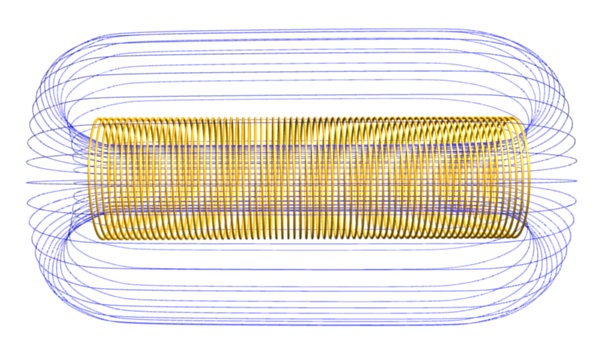
\includegraphics[height=0.5\textheight]{../figs/Solenoide.jpg}
\end{center}
\end{frame}

\begin{frame}[label={sec:orge2db12b}]{Bobina}
En un circuito magnético lineal el flujo es proporcional a la corriente:
\[
  \phi(t) = k \cdot i(t) \rightarrow   \frac{\mathrm{d}\phi(t)}{\mathrm{d} i(t)} = \frac{\phi(t)}{i(t)} = k
\]
En una bobina de \(N\) espiras la tensión autoinducida es:
\[
u(t) = N \cdot \frac{\mathrm{d}\phi(t)}{\mathrm{d} t}
\]

Combinando:
\[
u(t) = N \cdot \frac{\mathrm{d}\phi(t)}{\mathrm{d} i(t)} \cdot  \frac{\mathrm{d}i(t)}{\mathrm{d} t} \rightarrow u(t) = N \cdot \frac{\phi(t)}{i(t)} \cdot \frac{\mathrm{d}i(t)}{\mathrm{d} t}
\]
\begin{columns}
\begin{column}{0.7\columnwidth}
Por tanto, la ecuación de la bobina (autoinductancia \(L\), [H]):
\[
  \boxed{u(t) = L \cdot \frac{\mathrm{d}i(t)}{\mathrm{d} t}} \quad \boxed{L = N \cdot \frac{\phi(t)}{i(t)}}
\]
\end{column}
\begin{column}{0.3\columnwidth}
\begin{center}
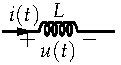
\includegraphics[height=0.2\textheight]{../figs/Bobina.pdf}
\end{center}
\end{column}
\end{columns}
\end{frame}





\section{Acoplamiento magnético}
\label{sec:orgc00d696}
\begin{frame}[label={sec:orgef9970a},plain]{}
\begin{center}
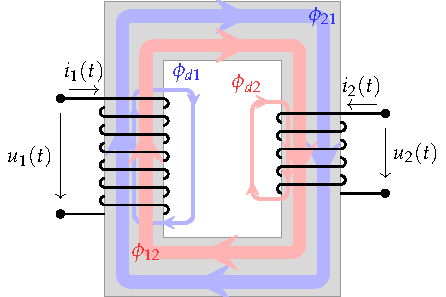
\includegraphics[height=0.9\textheight]{../figs/acoplamientoTikz.pdf}
\end{center}
\end{frame}

\begin{frame}[label={sec:orgf410bb6},plain]{}
\begin{center}
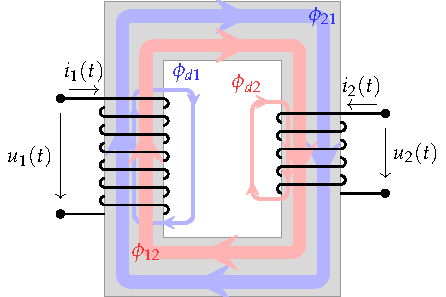
\includegraphics[height=0.55\textheight]{../figs/acoplamientoTikz.pdf}
\end{center}
\begin{center}
\(\phi_{ii}\): flujo producido por la bobina \(i\)

\(\phi_{ij}\): flujo recibido en bobina \(i\) producido por bobina \(j\)

\(\phi_{i}\): flujo total que atraviesa la bobina \(i\)
\end{center}
\begin{columns}
\begin{column}{0.5\columnwidth}
{\color{blue}\begin{align*}
  \phi_{11} &= \phi_{d1} + \phi_{21}\\
  \phi_{1} &= \phi_{11} + \phi_{12}
\end{align*}}
\end{column}
\begin{column}{0.5\columnwidth}
{\color{red}\begin{align*}
  \phi_{22} &= \phi_{d2} + \phi_{12}\\
  \phi_{2} &= \phi_{22} + \phi_{21}
\end{align*}}
\end{column}
\end{columns}
\end{frame}

\begin{frame}[label={sec:org4028ada},plain]{}
\begin{columns}
\begin{column}{0.5\columnwidth}
\begin{align*}
  u_1(t) = &N_1 \frac{\mathrm{d}\phi_1}{\mathrm{d}t} = \\
  &N_1 \frac{\mathrm{d}\phi_{11}}{\mathrm{d}t} + N_1 \frac{\mathrm{d}\phi_{12}}{\mathrm{d}t}
\end{align*}
\end{column}

\begin{column}{0.5\columnwidth}
\begin{align*}
  u_2(t) = &N_2 \frac{\mathrm{d}\phi_2}{\mathrm{d}t} = \\
  &N_2 \frac{\mathrm{d}\phi_{22}}{\mathrm{d}t} + N_2 \frac{\mathrm{d}\phi_{21}}{\mathrm{d}t}
\end{align*}
\end{column}
\end{columns}

\begin{center}
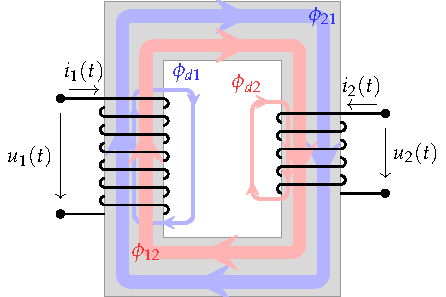
\includegraphics[height=0.45\textheight]{../figs/acoplamientoTikz.pdf}
\end{center}

\begin{center}
\(\phi_{ij}\): flujo recibido en bobina \(i\) producido por bobina \(j\)
\end{center}
\end{frame}
\begin{frame}[label={sec:orgeb727b5}]{Coeficientes de autoinducción e inducción mutua}
\begin{columns}
\begin{column}{0.4\columnwidth}
Coeficiente de autoinducción:
\begin{align*}
  L_1 &= N_1 \frac{\phi_{11}}{i_1}\\
  L_2 &= N_2 \frac{\phi_{22}}{i_2}
\end{align*}
Coeficiente de inducción mutua:
\begin{align*}
  M_{12} &= N_1 \frac{\phi_{12}}{i_2}\\
  M_{21} &= N_2 \frac{\phi_{21}}{i_1}
\end{align*}
\end{column}
\begin{column}{0.6\columnwidth}
\begin{center}
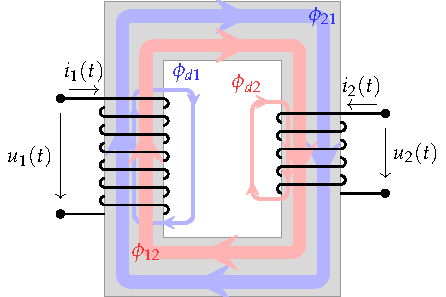
\includegraphics[height=0.7\textheight]{../figs/acoplamientoTikz.pdf}
\end{center}

\begin{center}
\(\phi_{ij}\): flujo recibido en bobina \(i\) producido por bobina \(j\)
\end{center}
\end{column}
\end{columns}
\end{frame}

\begin{frame}[label={sec:orgb03dd2f}]{Coeficiente de acoplamiento magnético}
\begin{columns}
\begin{column}{0.4\columnwidth}
Coeficiente de acoplamiento de la bobina 1:
\[
  k_1 = \frac{\phi_{21}}{\phi_{11}} = 1 - \frac{\phi_{d1}}{\phi_{11}} \leq 1
\]

Coeficiente de acoplamiento de la bobina 2:
\[
  k_2 = \frac{\phi_{12}}{\phi_{22}} = 1 - \frac{\phi_{d2}}{\phi_{22}} \leq 1
\]
\end{column}
\begin{column}{0.6\columnwidth}
\begin{center}
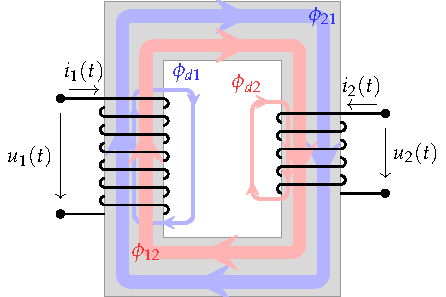
\includegraphics[height=0.7\textheight]{../figs/acoplamientoTikz.pdf}
\end{center}

\begin{center}
\(\phi_{ij}\): flujo recibido en bobina \(i\) producido por bobina \(j\)
\end{center}
\end{column}
\end{columns}
\end{frame}

\begin{frame}[label={sec:org42ee0ee}]{Coeficiente de inducción mutua}
Cuando el circuito magnético es \alert{lineal}:
\[
  \begin{rcases}
  M_{12} = M_{21} &= M\\
  k_1 = k_2 &= k    
  \end{rcases}
  \rightarrow \boxed{M = k \sqrt{L_1 \cdot L_2}} \qquad  k \leq 1
\]

Cuando el acoplamiento entre las dos bobinas es perfecto:
\[\left.
\begin{array}{cc}
  \phi_{d1} = 0 \rightarrow   \phi_{11} = \phi_{21}\\
  \phi_{d2} = 0 \rightarrow \phi_{22} = \phi_{12} 
  \end{array} \right\} \rightarrow k = 1
\]
\end{frame}

\begin{frame}[label={sec:orgc947c56}]{Resumen}
\begin{columns}
\begin{column}{0.4\columnwidth}
\begin{align*}
  L_1 &= N_1 \frac{\phi_{11}}{i_1}\\
  L_2 &= N_2 \frac{\phi_{22}}{i_2}
\end{align*}

\begin{align*}
  M &= N_1 \frac{\phi_{12}}{i_2}\\
    &= N_2 \frac{\phi_{21}}{i_1}
\end{align*}

\[
  M = k \sqrt{L_1 \cdot L_2}
\]
\end{column}

\begin{column}{0.6\columnwidth}
\begin{center}
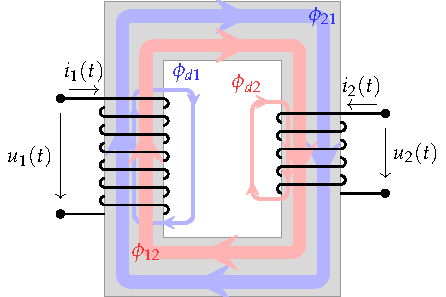
\includegraphics[height=0.7\textheight]{../figs/acoplamientoTikz.pdf}
\end{center}
\end{column}
\end{columns}
\end{frame}



\section{Representación Circuital}
\label{sec:orga6fe635}
\begin{frame}[label={sec:org536b6d9}]{Flujos del mismo sentido}
\begin{center}
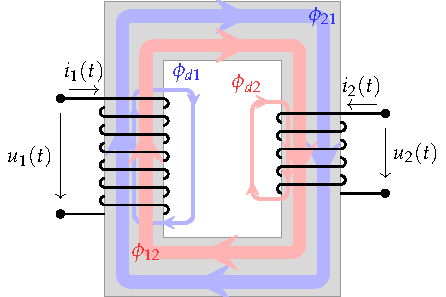
\includegraphics[height=0.75\textheight]{../figs/acoplamientoTikz.pdf}
\end{center}

\begin{center}
Las corrientes \(i_1\) e \(i_2\) producen flujos del mismo sentido.
\end{center}
\end{frame}


\begin{frame}[label={sec:orgaeba8b8}]{Flujos del mismo sentido: representación circuital}
\begin{columns}
\begin{column}{0.5\columnwidth}
\begin{center}
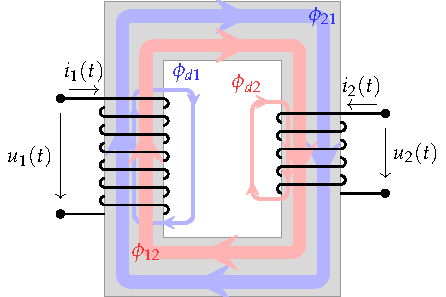
\includegraphics[width=.9\linewidth]{../figs/acoplamientoTikz.pdf}
\end{center}
\end{column}

\begin{column}{0.5\columnwidth}
\begin{center}
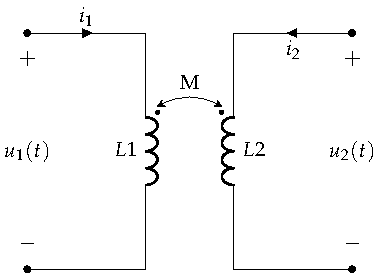
\includegraphics[width=.9\linewidth]{../figs/acoplamiento_circuito.pdf}
\end{center}
\end{column}
\end{columns}

\alert{Convención del punto}: se señala con un punto los terminales de las
bobinas por los que hay que introducir corrientes que producen flujos
del mismo sentido. Una corriente que entra por un terminal con punto
induce una tensión positiva en el otro terminal con punto.
\end{frame}
\begin{frame}[label={sec:orga203dd4}]{Flujos del mismo sentido: representación circuital}
\begin{columns}
\begin{column}{0.5\columnwidth}
\begin{center}
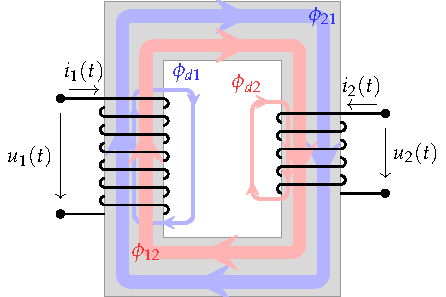
\includegraphics[width=.9\linewidth]{../figs/acoplamientoTikz.pdf}
\end{center}
\end{column}

\begin{column}{0.5\columnwidth}
\begin{center}
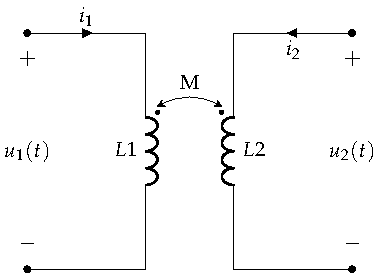
\includegraphics[width=.9\linewidth]{../figs/acoplamiento_circuito.pdf}
\end{center}
\end{column}
\end{columns}

\begin{align*}
  u_1(t) &= L_1 \frac{\mathrm{d}i_1(t)}{\mathrm{d}t} + M \frac{\mathrm{d}i_2(t)}{\mathrm{d}t}\\
  u_2(t) &= M \frac{\mathrm{d}i_1(t)}{\mathrm{d}t} + L_2 \frac{\mathrm{d}i_2(t)}{\mathrm{d}t}
\end{align*}
\end{frame}
\begin{frame}[label={sec:orgfea130f}]{Flujos contrapuestos}
\begin{center}
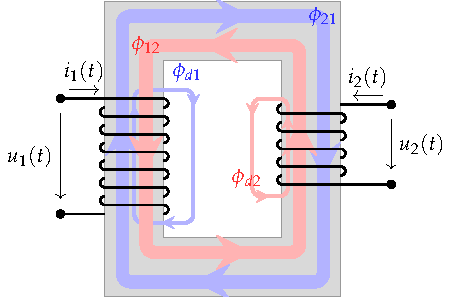
\includegraphics[height=0.75\textheight]{../figs/acoplamientoTikz_opuesto.pdf}
\end{center}

\begin{center}
Las corrientes \(i_1\) e \(i_2\) producen flujos de sentido contrario.
\end{center}
\end{frame}


\begin{frame}[label={sec:org5da4ca0}]{Flujos contrapuestos: representación Circuital}
\begin{columns}
\begin{column}{0.5\columnwidth}
\begin{center}
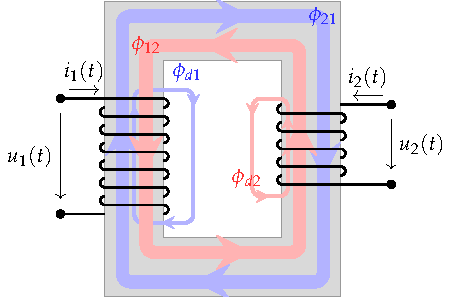
\includegraphics[width=.9\linewidth]{../figs/acoplamientoTikz_opuesto.pdf}
\end{center}
\end{column}


\begin{column}{0.5\columnwidth}
\begin{center}
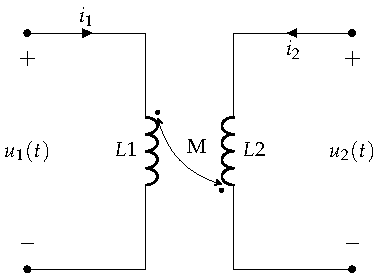
\includegraphics[width=.9\linewidth]{../figs/acoplamiento_circuito_opuesto.pdf}
\end{center}
\end{column}
\end{columns}
\alert{Convención del punto}: se señala con un punto los terminales de las
bobinas por los que hay que introducir corrientes que producen flujos
del mismo sentido. Una corriente que entra por un terminal con punto
induce una tensión positiva en el otro terminal con punto.
\end{frame}

\begin{frame}[label={sec:org591393b}]{Flujos contrapuestos: representación Circuital}
\begin{columns}
\begin{column}{0.5\columnwidth}
\begin{center}
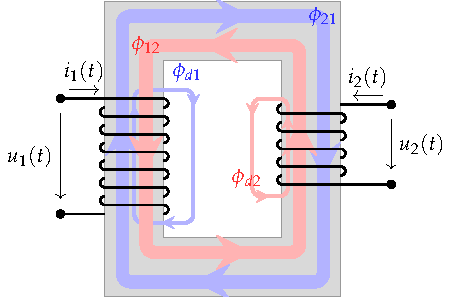
\includegraphics[height=0.45\textheight]{../figs/acoplamientoTikz_opuesto.pdf}
\end{center}
\end{column}

\begin{column}{0.5\columnwidth}
\begin{center}
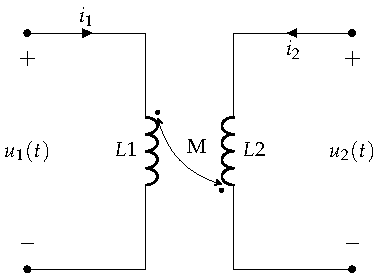
\includegraphics[height=0.45\textheight]{../figs/acoplamiento_circuito_opuesto.pdf}
\end{center}
\end{column}
\end{columns}
\begin{align*}
  u_1(t) &= L_1 \frac{\mathrm{d}i_1(t)}{\mathrm{d}t} - M \frac{\mathrm{d}i_2(t)}{\mathrm{d}t}\\
  u_2(t) &= - M \frac{\mathrm{d}i_1(t)}{\mathrm{d}t} + L_2 \frac{\mathrm{d}i_2(t)}{\mathrm{d}t}
\end{align*}
\end{frame}

\begin{frame}[label={sec:orgcd460f5}]{Corriente Alterna Sinusoidal}
\begin{columns}
\begin{column}{0.5\columnwidth}
\begin{center}
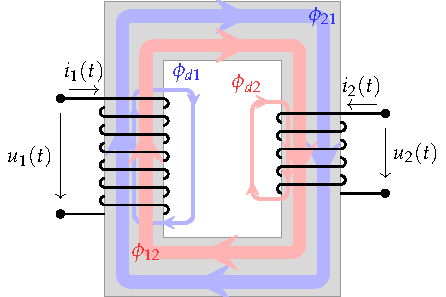
\includegraphics[height=0.45\textheight]{../figs/acoplamientoTikz.pdf}
\end{center}
\end{column}

\begin{column}{0.5\columnwidth}
\begin{center}
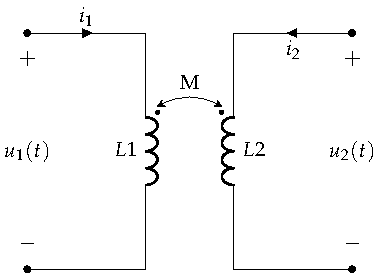
\includegraphics[height=0.45\textheight]{../figs/acoplamiento_circuito.pdf}
\end{center}
\end{column}
\end{columns}
\begin{align*}
  \overline{U}_1 &= j \omega L_1 \overline{I}_1 + j \omega M \overline{I}_2\\
  \overline{U}_2 &= j \omega M \overline{I}_1 + j \omega L_2 \overline{I}_2
\end{align*}
\end{frame}
\begin{frame}[label={sec:org7aba780}]{Corriente Alterna Sinusoidal}
\begin{columns}
\begin{column}{0.5\columnwidth}
\begin{center}
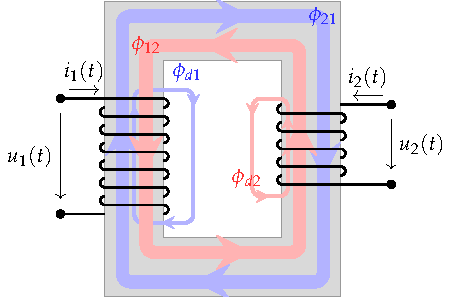
\includegraphics[height=0.45\textheight]{../figs/acoplamientoTikz_opuesto.pdf}
\end{center}
\end{column}

\begin{column}{0.5\columnwidth}
\begin{center}
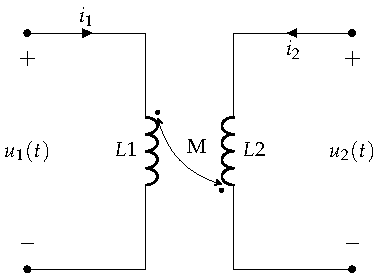
\includegraphics[height=0.45\textheight]{../figs/acoplamiento_circuito_opuesto.pdf}
\end{center}
\end{column}
\end{columns}
\begin{align*}
  \overline{U}_1 &= j \omega L_1 \overline{I}_1 - j \omega M \overline{I}_2\\
  \overline{U}_2 &= - j \omega M \overline{I}_1 + j \omega L_2 \overline{I}_2
\end{align*}
\end{frame}
\begin{frame}[label={sec:org60cc1fe}]{Ejemplo: acoplamiento de bobinas en serie}
\begin{center}
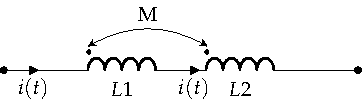
\includegraphics[height=0.2\textheight]{../figs/bobinas_serie.pdf}
\end{center}
\[
  \overline{U}_1 = (j \omega L_1 + j \omega M) \overline{I}
\]

\[
  \overline{U}_2 = (j \omega L_2 + j \omega M) \overline{I}
\]

\[
 \overline{U} = \overline{U}_1 + \overline{U}_2 \rightarrow \boxed{L = L_1 + L_2 + 2M}
\]
\end{frame}
\begin{frame}[label={sec:orgd4a4293}]{Ejemplo: acoplamiento de bobinas en serie}
\begin{center}
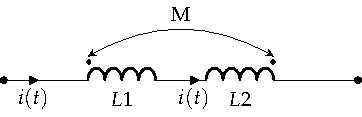
\includegraphics[height=0.2\textheight]{../figs/bobinas_serie_opuesto.pdf}
\end{center}
\[
  \overline{U}_1 = (j \omega L_1 - j \omega M) \overline{I}
\]

\[
  \overline{U}_2 = (j \omega L_2 - j \omega M) \overline{I}
\]

\[
 \boxed{L = L_1 + L_2 - 2M}
\]
\end{frame}
\end{document}
